% This is "sig-alternate.tex" V2.0 May 2012
% This file should be compiled with V2.5 of "sig-alternate.cls" May 2012
%
% This example file demonstrates the use of the 'sig-alternate.cls'
% V2.5 LaTeX2e document class file. It is for those submitting
% articles to ACM Conference Proceedings WHO DO NOT WISH TO
% STRICTLY ADHERE TO THE SIGS (PUBS-BOARD-ENDORSED) STYLE.
% The 'sig-alternate.cls' file will produce a similar-looking,
% albeit, 'tighter' paper resulting in, invariably, fewer pages.
%
% ----------------------------------------------------------------------------------------------------------------
% This .tex file (and associated .cls V2.5) produces:
%       1) The Permission Statement
%       2) The Conference (location) Info information
%       3) The Copyright Line with ACM data
%       4) NO page numbers
%
% as against the acm_proc_article-sp.cls file which
% DOES NOT produce 1) thru' 3) above.
%
% Using 'sig-alternate.cls' you have control, however, from within
% the source .tex file, over both the CopyrightYear
% (defaulted to 200X) and the ACM Copyright Data
% (defaulted to X-XXXXX-XX-X/XX/XX).
% e.g.
% \CopyrightYear{2007} will cause 2007 to appear in the copyright line.
% \crdata{0-12345-67-8/90/12} will cause 0-12345-67-8/90/12 to appear in the copyright line.
%
% ---------------------------------------------------------------------------------------------------------------
% This .tex source is an example which *does* use
% the .bib file (from which the .bbl file % is produced).
% REMEMBER HOWEVER: After having produced the .bbl file,
% and prior to final submission, you *NEED* to 'insert'
% your .bbl file into your source .tex file so as to provide
% ONE 'self-contained' source file.
%
% ================= IF YOU HAVE QUESTIONS =======================
% Questions regarding the SIGS styles, SIGS policies and
% procedures, Conferences etc. should be sent to
% Adrienne Griscti (griscti@acm.org)
%
% Technical questions _only_ to
% Gerald Murray (murray@hq.acm.org)
% ===============================================================
%
% For tracking purposes - this is V2.0 - May 2012

\documentclass{sig-alternate}

% \usepackage[scaled=0.92]{helvet}   % set Helvetica as the sans-serif font
% \renewcommand{\rmdefault}{ptm}     % set Times as the default text font

%\usepackage[amssymbols,subscriptcorrection,slantedGreek,nofontinfo]{mtpro2}
%\usepackage[lite,subscriptcorrection,slantedGreek,nofontinfo]{mtpro2}

\usepackage{framed}
\usepackage{booktabs}

% references for sections etc.
\newcommand{\mysec}[1]{Section~\ref{sec:#1}}
\newcommand{\myapp}[1]{Appendix~\ref{app:#1}}
\newcommand{\myeq}[1]{Equation~\ref{eq:#1}}
\newcommand{\myeqp}[1]{Eq.~\ref{eq:#1}}
\newcommand{\mychap}[1]{Chapter~\ref{chap:#1}}
\newcommand{\myfig}[1]{Figure~\ref{fig:#1}}

% math conveniences
\newcommand{\g}{\,\vert\,}
\newcommand{\E}{\textrm{E}}
\newcommand{\vct}[1]{\textbf{#1}}
\newcommand{\realline}{\mathbb{R}}
\newcommand{\indpt}{\protect\mathpalette{\protect\independenT}{\perp}}
\def\independenT#1#2{\mathrel{\rlap{$#1#2$}\mkern2mu{#1#2}}}
\newcommand{\h}[1]{\textrm{H}\left( #1 \right)}
\newcommand{\half}{\frac{1}{2}}
\newcommand{\new}{\textrm{new}}
\newcommand{\discrete}{\textrm{Discrete}}
\newcommand{\Bern}{\textrm{Bern}}
\newcommand{\DP}{\textrm{DP}}
\newcommand{\GP}{\textrm{GP}}
\newcommand{\Bet}{\textrm{Beta}}

\newcommand{\ddx}[1]{\frac{\partial}{\partial #1}}
\newcommand{\dfdx}[2]{\textstyle \frac{\partial #1}{\partial #2}}

\newcommand{\poisson}{\textrm{Poisson}}
\newcommand{\mult}{\textrm{Mult}}
\newcommand{\dir}{\textrm{Dirichlet}}
\newcommand{\gam}{\textrm{Gamma}}
\newcommand{\shape}{\textrm{shp}}
\newcommand{\rate}{\textrm{rte}}


\begin{document}
%
% --- Author Metadata here ---
%\conferenceinfo{WOODSTOCK}{'97 El Paso, Texas USA}
%\CopyrightYear{2007} % Allows default copyright year (20XX) to be over-ridden - IF NEED BE.
%\crdata{0-12345-67-8/90/01}  % Allows default copyright data (0-89791-88-6/97/05) to be over-ridden - IF NEED BE.
% --- End of Author Metadata ---

\title{Scalable Recommendation with Poisson Factorization}

%
% You need the command \numberofauthors to handle the 'placement
% and alignment' of the authors beneath the title.
%
% For aesthetic reasons, we recommend 'three authors at a time'
% i.e. three 'name/affiliation blocks' be placed beneath the title.
%
% NOTE: You are NOT restricted in how many 'rows' of
% "name/affiliations" may appear. We just ask that you restrict
% the number of 'columns' to three.
%
% Because of the available 'opening page real-estate'
% we ask you to refrain from putting more than six authors
% (two rows with three columns) beneath the article title.
% More than six makes the first-page appear very cluttered indeed.
%
% Use the \alignauthor commands to handle the names
% and affiliations for an 'aesthetic maximum' of six authors.
% Add names, affiliations, addresses for
% the seventh etc. author(s) as the argument for the
% \additionalauthors command.
% These 'additional authors' will be output/set for you
% without further effort on your part as the last section in
% the body of your article BEFORE References or any Appendices.

\numberofauthors{3}

% %  in this sample file, there are a *total*
% of EIGHT authors. SIX appear on the 'first-page' (for formatting
% reasons) and the remaining two appear in the \additionalauthors section.
%
\author{}
% You can go ahead and credit any number of authors here,
% e.g. one 'row of three' or two rows (consisting of one row of three
% and a second row of one, two or three).
%
% The command \alignauthor (no curly braces needed) should
% precede each author name, affiliation/snail-mail address and
% e-mail address. Additionally, tag each line of
% affiliation/address with \affaddr, and tag the
% e-mail address with \email.
%
% 1st. author

%% \alignauthor
%% Prem Gopalan\\
%% \affaddr{Princeton University}\\
%% \affaddr{35 Olden Street}\\
%% \affaddr{Princeton, NJ}\\
%% \email{pgopalan@cs.princeton.edu}
%% % 2nd. author
%% \alignauthor
%% Jake M. Hofman \\
%% \affaddr{Microsoft Research}\\
%% \affaddr{641 Sixth Avenue, Floor 7}\\
%% \affaddr{New York, NY}\\
%% \email{jmh@microsoft.com}
%% % 3rd. author
%% \alignauthor
%% David M. Blei \\
%% \affaddr{ Princeton University}\\
%% \affaddr{35 Olden Street}\\
%% \affaddr{Princeton, NJ}\\
%% \email{blei@cs.princeton.edu}
%% }
\maketitle

\begin{abstract}
We develop hierarchical Poisson matrix factorization (HPF) for
recommendation.  HPF models sparse user behavior data, large user/item
matrices where each user has provided feedback on only a small subset
of items.  HPF handles both explicit ratings, such as a number of
stars, or implicit ratings, such as views, clicks, or purchases.  We
develop a variational algorithm for approximate posterior inference
that scales up to massive data sets, and we demonstrate its
performance on a wide variety of real-world recommendation
problems--users rating movies, users listening to songs, users reading
scientific papers, and users reading news articles.  Our study reveals
that hierarchical Poisson factorization definitively outperforms
previous methods, including nonnegative matrix factorization, topic
models, and state-of-the-art probabilistic matrix factorization
techniques.
\end{abstract}
%% % A category with the (minimum) three required fields
%% \category{H.4}{Information Systems Applications}{Miscellaneous}
%% %A category including the fourth, optional field follows...
%% \category{D.2.8}{Software Engineering}{Metrics}[complexity measures, performance measures]
%% \terms{Theory}

%% \keywords{ACM proceedings, \LaTeX, text tagging}


\section{Introduction}

Recommendation systems are a vital component of the modern Web.  They
help readers effectively navigate otherwise unwieldy archives of
information and help websites direct users to items---movies,
articles, songs, apps---that they will like.  A recommendation system
is built from user behavior data, historical data about which items
each user has consumed.  First, a statistical machine learning
algorithm is used to uncover behavioral patterns that reveal the
various types of users and the items they tend to like.  Then, the
system exploits these discovered patterns to recommend future items to
its users.

As an example, Figure 1 illustrates movie recommendation for a user
$U$ from the MovieLens data set~\cite{Herlocker:1999}.  This data set
is a large sparse matrix where rows are people and columns are movies.
Each entry of the matrix (indexed by a user and a movie) contains the
rating that the user gave to the movie, or a zero if she has not seen
it. The list of movies at the top of the
\myfig{movielens-illustration} shows that user $U$ enjoys various
types of drama movies (such as the war drama ``Breaker Morant'' and
the romantic drama ``Leaving Las Vegas''). Of course, she has only
seen a handful of the available movies, and the goal of a
recommendation system is to suggest other movies.  The list of movies
at the bottom of the figure was suggested by our algorithm. It
includes other war drama movies (such as "Apocalypse Now") and other
romantic drama (such as "Breakfast at Tiffany's").  In this paper, we
develop a new algorithm for building recommendation systems that is
both more efficient and performs better than the existing
state-of-the-art.

\begin{figure*}[th]
\centering
\caption{The top 5 movies in each of the top 4 components of the user
  $U$ illustrated in Fig~\ref{fig:movielens-illustration}.}
\vspace{0.1cm}
\small
\begin{tabular}{c}
\toprule
\bf{``Drama, Romance''}\\
\midrule
Breakfast at Tiffany's\\
Casablanca\\
The Graduate\\
Shakespeare in Love\\
The African Queen\\
\bottomrule
\end{tabular}
\begin{tabular}{c}
\toprule
\bf{``Drama''}\\
\midrule
Jean de Florette\\
Manon of the Spring\\
Diva\\
The Return of Martin Guerre\\
Blue Velvet\\
\bottomrule
\end{tabular}
\begin{tabular}{c}
\toprule
\bf{``Children's Drama''}\\
\midrule
The Secret Garden\\
The Secret of Roan Inish\\
A Little Princess\\
Fly Away Home\\
Black Beauty\\
\bottomrule
\end{tabular}
\begin{tabular}{c}
\toprule
\bf{``Drama, War''}\\
\midrule
The Bridge on the River Kwai\\
The Right Stuff\\
Patton\\
The Killing Fields\\
Gandhi\\
\bottomrule
\end{tabular}

\end{figure*}

\begin{figure}
\centering
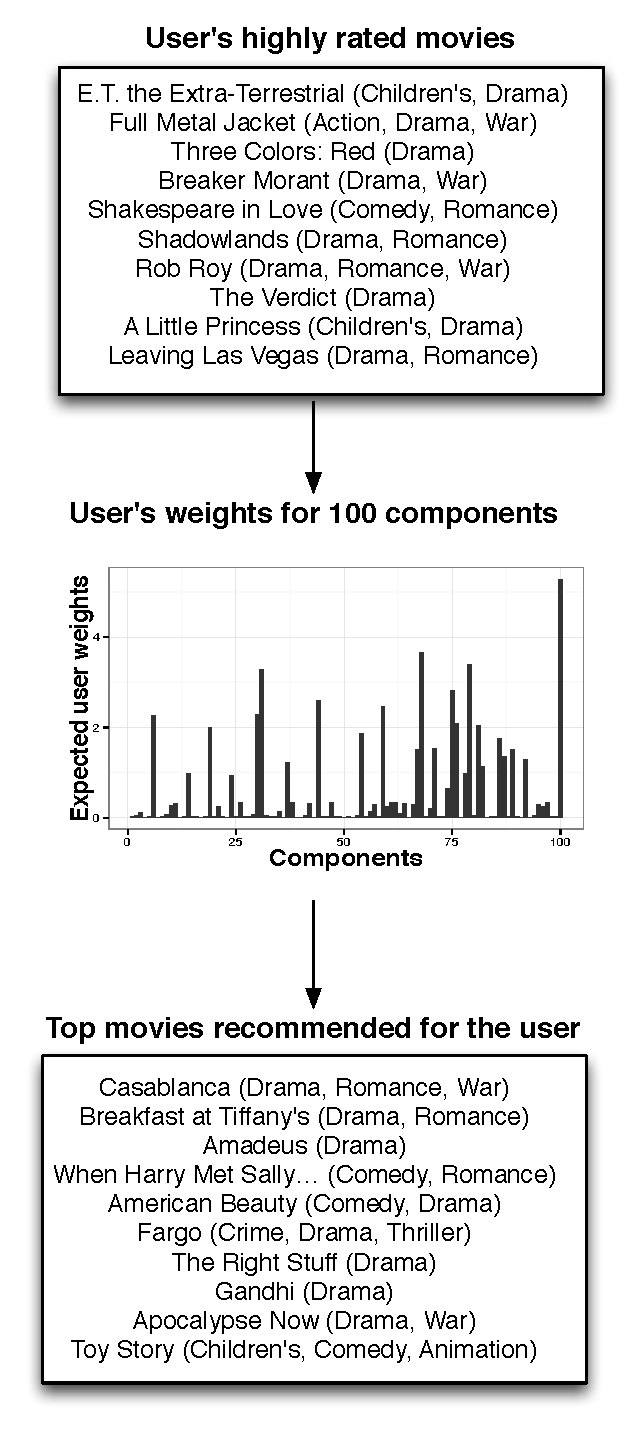
\includegraphics[width=0.8\columnwidth]{figures/movielens-user2.pdf}\\
\caption{An illustration showing a subset of the highly rated movies
  of a selected user $U$ in the MovieLens data set~\cite{Herlocker:1999},
  and a subset of the movies in the top 15 recommended to the user by
  our algorithm. The expected user's $K$-vector of weights $\theta_u$,
  inferred by our algorithm is shown. In our analysis, $K$ was set to
  100.}
\label{fig:movielens-illustration}
\end{figure}


%%
%%\begin{figure}
%%\centering
%%\includegraphics[width=0.8\columnwidth]{figures/movielens-user.pdf}\\
%%\includegraphics[width=0.8\columnwidth]{figures/movielens-item.pdf}\\
%%\caption{The weights of the randomly chosen user $U$ (Top) in the
 %% movielens data set and the weights of her top recommended movie
  %%\emph{Shakespeare in Love} (Bottom) are shown. User $U$ views a
  %%variety of movies, and her weights span a range of factor. User $U$
  %%had 184 views in the data set of movies ranging from Drama, Comedy,
  %%Thriller to Musical. Of these movies, 126 were either 4 or 5
  %%stars. Movies are generally characterized by a sparse set of
  %%factors.}
%%\end{figure}


Currently, the workhorse method for recommendation systems is matrix
factorization (MF). MF represents users and items with low dimensional
vectors and computes the affinity between a user and item (that is,
whether the user will like it) with the dot product of their
respective representations.  MF is typically fit with squared loss,
where the algorithm finds representations that minimize the squared
difference between the predicted value and the observed rating.  (This
corresponds to a Gaussian model of the
data~\cite{Salakhutdinov:2008}.)  MF has been extended in many ways to
implement modern recommendation
systems~\cite{Dror:2012,Koren:2008,Rendle:2009,Stern:2009p9238}.

However, the assumptions behind traditional MF are fundamentally
flawed when analyzing real-world user behavior data.  In real-world
data, each user has only rated a small subset of the large population
of available items. An item a user did \textit{not} rate can arise in
two ways: either she considered it and chose not to rate it or she did
not consider it at all.  Each user has a limited budget (of money,
attention, or time) and therefore most of the unrated items in the
matrix arise from users not considering (as opposed to actively disliking) them.

The issue with traditional MF is that it treats all the missing cells
as observations, as though every user has enough attention to consider
every available item and decide whether to rate it.  Thus, the missing
cells are seen as evidence for users not liking the items, and this
significantly biases the learned representations.  To address the
problem, researchers have patched MF in a variety of ways, for example
by artificially down-weighting the contribution of the unrated items~\cite{Hu:2008p9402},
by sub-sampling from the unrated items to give equal weight to the
rated items~\cite{Gantner:2012p9364,Dror:2012a}, or by explicitly modeling the unrated
items as missing data~\cite{Paquet:2013p9197}.

This issue is particularly critical when analyzing binary data, such
as product purchases or webpage clicks.  Binary behavior data records
whether each user consumed an item but does provide a rating.
Building recommendation systems from such matrices is known as
one-class collaborative filtering or recommendation with implicit
feedback~\cite{Hu:2008p9402,Paquet:2013p9197}.

In this paper, we develop a Bayesian Poisson factorization model as an
alternative to traditional MF for building recommendation systems.
Our model implicitly assumes that each user has a limited budget with
which to consume items~\cite{Goodhardt:1984}, and thus an item that a
user has consumed provides a stronger signal about her preferences
than an item that a user has not consumed.  With several kinds of data
sets---users rating movies~\cite{Herlocker:1999,Koren:2009}, users
listening to songs~\cite{Bertin-Mahieux:2011}, and users reading
scientific papers~\cite{Jack:2010}---we demonstrate that Poisson
factorization leads to better recommendations than both traditional
matrix factorization and its variants that adjust for sparse data.

Furthermore, Poisson factorization is computationally more efficient
than traditional MF.  Most algorithms for fitting MF must iterate over
all user/item pairs, which is expensive for even modestly-sized user
behavior matrices and cannot take advantage of the sparsity of the
data~\cite{Hu:2008p9402}.  (To address this issue, practical applications of matrix
factorization rely on stochastic optimization~\cite{Mairal:2010}.)  In
this paper, we derive efficient variational inference algorithms for
Poisson factorization that take advantage of the sparsity of the
data. Our algorithms need only iterate over the non-zero entries of
the user behavior matrix.  This lets us handle data at a scale that
basic (non-stochastic) MF algorithms cannot handle.



\begin{figure*}[t!]
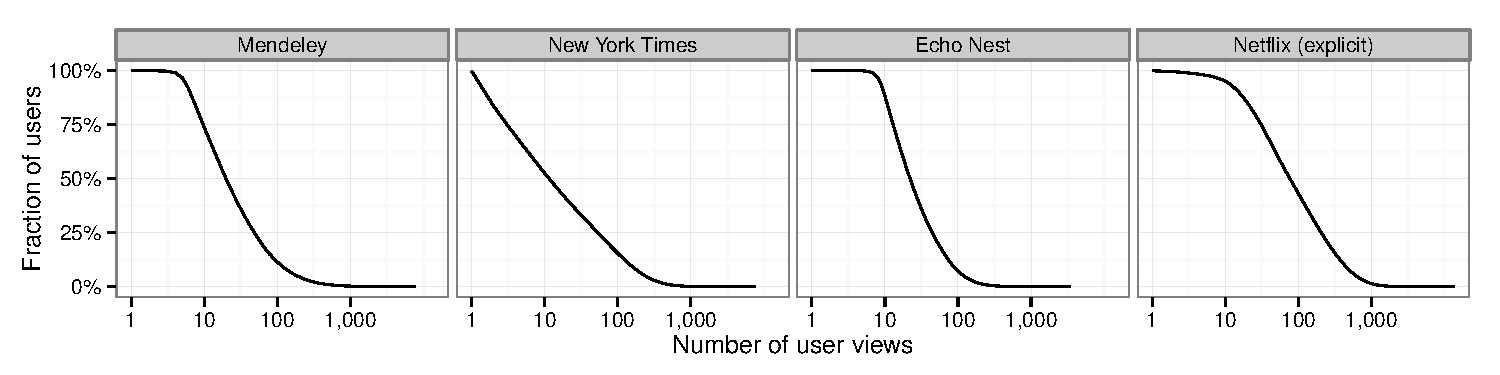
\includegraphics[width=\textwidth]{figures/user_activity_cdf.pdf}
\caption{Empirical complimentary cumulative distributions of user activity on each dataset. Each curve shows the fraction of users who have consumed at least a given number of items. For instance, slightly less than half of all Netflix users have viewed at least 100 movies.}
\label{fig:marginals}
\end{figure*}

%% \begin{figure*}[t!]
%% 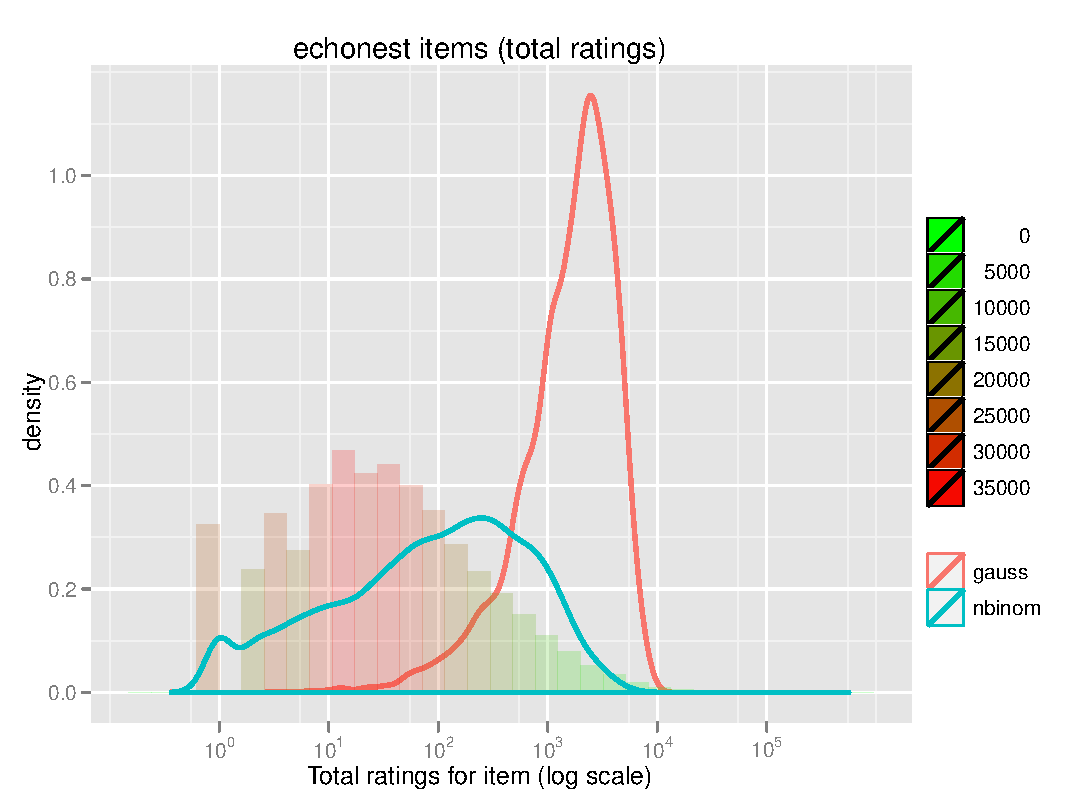
\includegraphics[width=0.33\textwidth]{figures/marginals/echonest.pdf}
%% 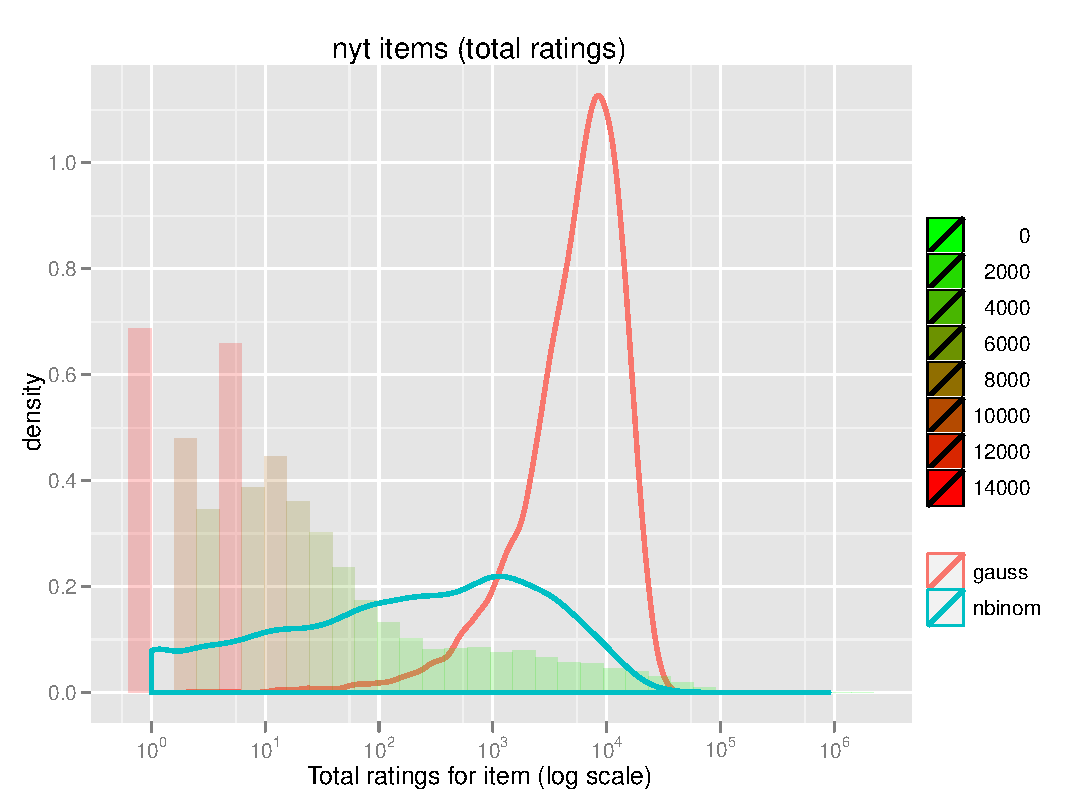
\includegraphics[width=0.33\textwidth]{figures/marginals/nyt.pdf}
%% 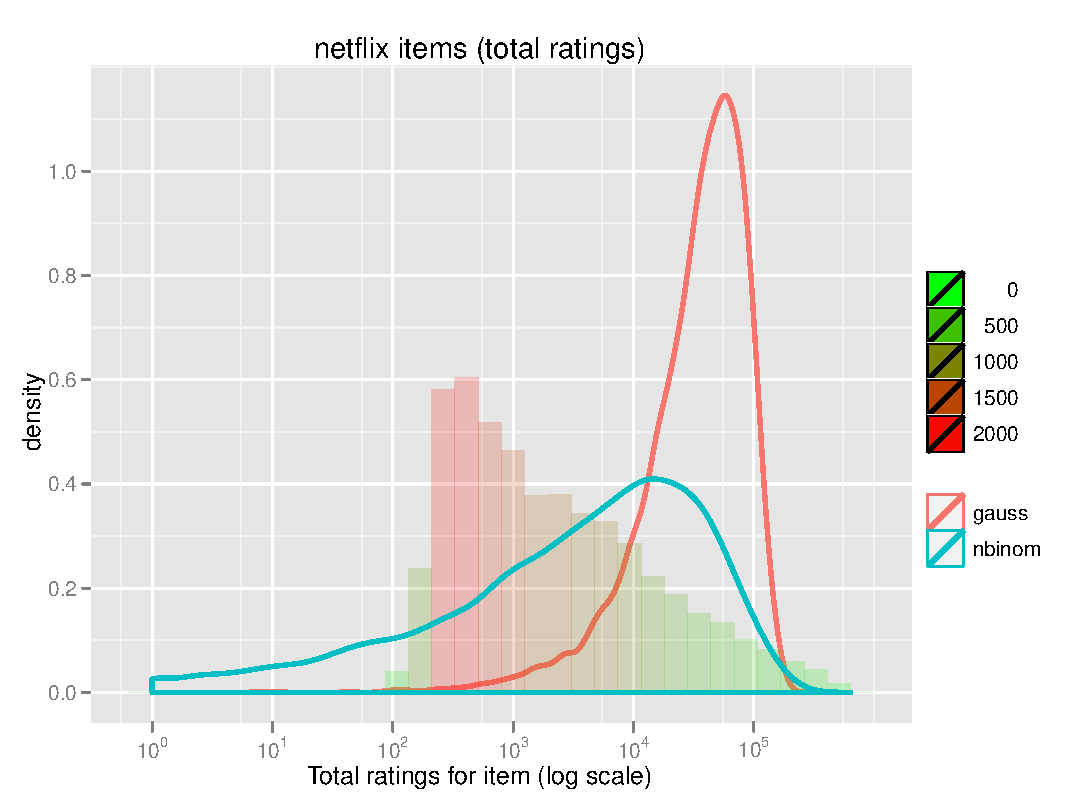
\includegraphics[width=0.33\textwidth]{figures/marginals/netflix.pdf}
%% \caption{Empirical distribution of item popularity on real datasets,
%%   with fitted negative binomial and Gaussian distributions. The
%%   distributions were fit using maximum likelihood estimation. The
%%   negative binomial places significant probability mass on the left
%%   tail, i.e., items with few ratings. The colored bars show that such
%%   items are the most frequent. In contrast, the Gaussian distribution
%%   places negligible mass on the left tail and mainly captures popular
%%   items. The mode of the negative binomial distribution is also closer
%%   to the empirical mode than the Gaussian distribution.}
%% \label{fig:marginals}
%% \end{figure*}

% prem: no longer use stochastic 

%% Further speed-ups using stochastic variational
%% inference~\cite{Hoffman:2013} let us fit Poisson factorization models
%% to massive data.


\section{Poisson Recommendation}
\label{sec:model}

% !!! review the Gamama and Poisson near the generative process.
% !!! make n_u and n_i the sums
% !!! somewhere we need to make clear how our notation works

We are given data about users and items.  Each user has consumed and
possibly rated a set of items.  The observation $y_{ui}$ is the rating
that user $i$ gave to item $j$, or zero if no rating was given.  (In
simple consumer data, $y_{ui}$ equals one if user $u$ consumed item
$i$ and zero otherwise.)  User behavior data, such as purchases,
ratings, clicks, ``likes'', or ``check ins'', are typically sparse.
Most of the values of the matrix $y$ are zero.

We model this data with factorized Poisson
distributions~\cite{Canny:2004}. Each user $u$ and each item $i$ is
associated with a $K$-vector of positive weights, $\theta_u$ and
$\beta_i$ respectively.  (The number $K$ is fixed in advance.)  The
user/item observation $y_{ui}$ is modeled with a Poisson parameterized
by the inner product of the user's and item's weights $y_{ui} \sim
\poisson(\theta_u^\top \beta_i)$.  This is a variant of
probabilistic matrix factorization~\cite{Salakhutdinov:2008a} but
where each user and item's weights are positive~\cite{Lee:1999}---we
place Gamma priors on them--- and where the Poisson likelihood
replaces the Gaussian likelihood.

% dmb: jake cites something below
% dmb: also cite "The Dirichlet", old marketing paper

This Poisson model has good properties when modeling user/item data.
It implicitly assumes that each user consumes a negative-binomial number of
items---a heavy-tailed distribution that is known to fit user activity
well~\cite{Goodhardt:1984}--and this forces it to down-weight the
contribution of the items that each user did not consume. The reason
is that the model has two ways of explaining that a user does not
consume an item: either she is not interested in it or she would be
but has already consumed her allotted negative-binomial number.  In
contrast, a user that consumes an item must be interested in it.
Thus, the model benefits more from making a consumed user/item pair
more similar than making an unconsumed user/item pair less similar.

Classical matrix factorization is based on Gaussian likelihoods (i.e.,
squared loss), which gives equal weight to consumed and unconsumed
items.  Consequently, when faced with a sparse matrix, matrix
factorization places more total emphasis on the unconsumed user/item
pairs.  To address this, researchers have patched the model in complex
ways, for example, by including per-observation
confidences~\cite{Koren:2009} or considering all zeroes to be hidden
variables~\cite{Paquet:2013p9197}.  Poisson factorization more naturally solves this
problem by capturing each user's rate of consumption.

As an example, consider two similar science fiction movies, ``Star
Wars'' and ``The Empire Strikes Back'', and consider a user who has
seen one of them.  The Gaussian model pays an equal penalty for making
the user similar to these items as it does for making the user
different from them---with quadratic loss, seeing ``Star Wars'' is
evidence for liking science fiction, but not seeing ``The Empire
Strikes Back'' is evidence for disliking it.  The Poisson model,
however, will prefer to bring the user's latent weights closer to the
movies' weights because it favors the information from the user
watching ``Star Wars''. Further, because the movies are similar, this
increases the Poisson model's predictive score that a user who watches
``Star Wars'' will also watch ``The Empire Strikes Back''.


\subsection{The generative model}

The generative process of the hierarchical Poisson factorization model
(HPF) is as follows:
\begin{enumerate}
\item For each user $u$, choose activity
  \begin{equation*}
    \xi_u \sim \gam(a', b').
  \end{equation*}
\item For each user $u$ and each component $k$, choose weight
  \begin{equation*}
    \theta_{uk} \sim \gam(a, \xi_u).
  \end{equation*}
\item For each item $i$, choose popularity
  \begin{equation*}
    \eta_i \sim \gam(c', d').
  \end{equation*}
\item For each item $i$ and each component $k$, choose weight
  \begin{equation*}
    \beta_{ik} \sim \gam(c, \eta_i).
  \end{equation*}
\item For each user $u$ and item $i$, choose rating
  \begin{equation*}
    y_{ui} \sim \poisson(\theta_u^\top \beta_i).
  \end{equation*}
\end{enumerate}
The model places a \gam~prior on each of the \gam~rate parameters
governing user and item weights. The prior on $\xi_u$ captures the
uncertainty around user $u$'s consumption rate or activity; the prior
on $\eta_i$ captures the uncertainty around item $i$'s popularity
among users. 

We also study a sub-class of the HPF where we fix the rate parameter
$\xi_u$ for each user, and the rate parameter $\eta_i$ for each
item. We call this model the Bayesian Poisson Factorization (BPF)
model.

The HPF model is more powerful than the BPF because it allows for the
sharing of statistical strength. In the HPF, for example, learning
about the number of items consumed by one set of users provides weak,
indirect evidence relevant to other users consumption. This can
improve predictions, especially for users with little activity. A
similar argument favors hierarchy over item popularities. In the HPF,
we fix the shape parameters and share them across users and items. For
a large shape, the weights will tend to have similar magnitude, and
the representations will be dense. In contrast, a small shape will
result in a sparse representation.  Finally, the \gam~prior is
conjugate to the \gam~distribution with fixed shape governing the
weights. This results in a computationally efficient algorithm.

%% explain the computational efficiency obtained?
 
The posterior distribution of the latent variables $p(\theta, \beta,
\xi, \eta \g y)$ embeds users and items in a latent space of
$K$-dimensional positive vectors. 

We use the HPF to recommend items to users by predicting which of the
unconsumed items each will like.  We rank each user's unconsumed items
by their posterior expected Poisson parameters,
\begin{equation}
  \label{eq:score}
  \textrm{score}_{ui} = \E[\theta_u^\top \beta_i \g y].
\end{equation}
This amounts to asking the model to rank by probability which of the
presently unconsumed items each user will likely consume in the
future.

With these details in place, we highlight two statistical properties of the
model. First, we mentioned above that the marginal distribution of
each user's ratings is a negative binomial.  Let $y_{u} = \sum_{i}
y_{ui}$ be the sum of the ratings for user $u$.  Since each of the
terms in the sum is a Poisson distribution with rate $\theta_u^\top
\beta_i$, the sum is itself a Poisson random
variable~\cite{Johnson:2005}.
\begin{equation}
  y_u \sim \poisson\left(\theta_u^\top (\textstyle \sum_{i} \beta_{i})\right).
\end{equation}
Holding the item weights fixed, note that the rate of this Poisson is
a sum of scaled Gamma random variables $\beta_{ik} \theta_{uk}$, which is
itself a Gamma variable~\cite{Norman:1994}.  Thus the marginal
distribution of $y_u$ is from an integrated Gamma-Poisson
distribution, which is a negative binomial~\cite{Gelman:1995}.

% dmb: above, maybe add a comment above that this is a heavy-tailed
% realistic distribution for consumer data.  cite goodhardt 1984
% again.

Second, the likelihood of the observed data depends only on the
consumed items, that is, the non-zero elements of the user/item matrix
$y$.  Given the latent variables $\theta_u$ and $\beta_i$, the Poisson
distribution of $y_{ui}$ is
\begin{equation}
  p(y_{ui} \g \theta_u, \beta_i) =
  \left(\theta_u^\top \beta_i\right)^y
  \exp\left\{-\theta_u^\top \beta_i \right\} / y_{ui}!
\end{equation}
Recall the elementary fact that $0! = 1$.  The log probability of the
complete matrix $y$ is
\begin{align}
  \log p(y \g \theta, \beta) =
  & \left(\textstyle \sum_{\{y_{ui} > 0\}}
    y_{ui} \log (\theta_u^\top \beta_i) - \log y_{ui}!
  \right) \\
  & -
  \left(\textstyle\sum_{u} \theta_u\right)^\top \left(\textstyle
    \sum_{i} \beta_i\right).
\end{align}
That this likelihood depends only on the non-zero elements facilitates
inference with sparse matrices.  In contrast, classical matrix
factorization methods, especially when applied to
massive data sets, must address the zeros either through
sub-sampling~\cite{Dror:2012a} or approximation~\cite{Hu:2008p9402}.

%% Finally, we follow the literature on recommendation systems which
%% finds that per-item and per-user bias terms significantly help
%% performance. These terms capture universally popular items and
%% frequently consuming users.  For simplicity, we present our algorithms
%% without these terms, but we include them in our empirical study. The
%% corresponding changes to the algorithm are minimal.\footnote{In
%% particular, we include these biases with dummy factors that are always
%% equal to one for each user and each item.}

\subsection{Related work}

The roots of Poisson factorization come from nonnegative matrix
factorization~\cite{Lee:1999}, where the objective function is
equivalent to a factorized Poisson likelihood.  Placing a Gamma prior
on the user weights gives the GaP model~\cite{Canny:2004}, which was
developed as an alternative text model to latent Dirichlet allocation
(LDA)~\cite{Blei:2003b}.

A difference between our treatment and GaP is that GaP fits the item
weights with maximum likelihood via the expectation maximization
algorithm.  Our model places Gamma priors on these weights (step 2,
above) and we approximate the full posterior with variational
inference.  Placing priors on both sets of weights further regularizes
the model and lets us use the same inferential machinery in both
user-space and item-space.  

% prem: removed reference to stochastic inference
%       we should add this in future work/discussion
%% Furthermore, using variational inference opens the door to scaling to
%% massive data sets, even larger than the data sets we analyze in this
%% paper, using stochastic variational inference~\cite{Hoffman:2013} (see
%% \mysec{inference}).

We note that GaP was developed as an alternative to LDA. In Appendix
A, we show that LDA can be reinterpreted as an instance of Poisson
factorization where we condition on the user counts and use an
alternative prior on the item weights.  (This connection was
previously unknown.)

Independently of GaP, Bayesian Poisson factorization has been studied
in the signal processing community for performing source separation
from spectrogram data~\cite{Cemgil:2009,Hoffman:2012}.  This research
includes variational approximations to the posterior, though the
issues and details around spectrogram data differ significantly from
user behavior data we consider and our derivation below (based on
auxiliary variables) is more direct.  As future work, the methods
developed here could lead to improved methods for massive simultaneous
analysis of audio spectrograms. In the context of network data, a
Poisson model of overlapping communities was described by the authors
of ~\cite{Ball:2011}. As with GaP, this model is unregularized and the
authors fit the model with maximum likelihood via expectation
maximization.

We discuss further differences between our method and previous work on
matrix factorization in the empirical results below.

% !!! add reference to canny's click data
% !!! add reference to SIGIR
XXX \cite{Marlin:2009,Marlin:2012,Elkan:2008}

\section{Variational Inference}
\label{sec:inference}

The key computation for the HPF is the posterior distribution of the
user weights $\theta_{uk}$, item weights $\beta_{ik}$, user activity
$\xi_{u}$ and item popularity $\eta_i$ given an observed matrix
of user behavior $y$,
\begin{equation*}
  p(\theta, \beta, \xi, \eta \g y) = \frac{p(\theta | \xi) p(\xi)
    p(\eta) p(\beta | \eta) p(y \g \theta, \beta, \xi, \eta)}
  {\int_{\theta} \int_{\xi} \int_{\eta} \int_{\beta} p(\theta |
    \xi) p(\xi) p(\beta) p(\beta | \eta) p(y \g \theta, \beta, \xi, \eta)}.
\end{equation*}
We need the posterior to form recommendations with the posterior
expectations in \myeq{score}.

As for many Bayesian models of interest, however, the posterior is
intractable to compute exactly.  The problem is with the denominator,
which is the marginal probability of the observed matrix and involves
a complicated and high-dimensional integral.  In this section, we show
how to efficiently approximate the posterior with mean-field
variational inference.

Variational inference is a general strategy for approximating
posterior distributions in complex probabilistic
models~\cite{Jordan:1999,Wainwright:2008}.  Variational inference
algorithms posit a family of distributions over the hidden variables,
indexed by free ``variational'' parameters, and then find the member
of that family that is closest in KL divergence to the true posterior.
(The form of the family is chosen to make this optimization possible.)
Thus, variational inference turns the inference problem into an
optimization problem.  Variational algorithms tend to scale better
than alternative sampling-based approaches, like Monte Carlo Markov
chain sampling, and have been deployed to solve many applied problems
with complex models, including large-scale recommendation~\cite{Paquet:2013p9197}.

We develop mean-field variational inference algorithm for the HPF.  We
first describe the mean-field variational family and the corresponding
variational objective.  We then derive a batch algorithm that fits the
variational distribution by repeatedly cycling through the non-zero
data and updating its estimates of the latent representations. The
simple structure of the algorithm lets us scale our approach to data
sets like the full Netflix data (18,000 movies and 480,000 users) on a
single CPU.

% prem: remove stochastic
%% Finally, we develop a scalable stochastic variational inference
%% algorithm for massive data.  This algorithm repeatedly subsamples
%% users from the matrix and updates its estimates of the latent
%% representations.  

Before beginning these derivations, however, we give an alternative
formulation of the model in which we add a layer of latent variables.
These auxiliary variables allow us to take advantage of some general
results for variational
algorithms~\cite{Ghahramani:2001,Hoffman:2013}.  For each user and
item we add $K$ latent variables $z_{uik} \sim \poisson(\theta_{uk}
\beta_{ik})$, which are integers that sum to the user/item value
$y_{ui}$.  A sum of Poisson random variables is itself a Poisson with
rate equal to the sum of the rates.  Thus, these new latent variables
preserve the marginal distribution of the observation, $y_{ui} \sim
\poisson(\theta_{u}^\top \beta_{i})$.  These variables can be thought
of as the contribution from component $k$ to the total observation
$y_{ui}$.  Note that when $y_{ui} = 0$, these auxiliary variables are
not random---the posterior distribution of $z_{ui}$ will place all its
mass on the zero vector.  Consequently, our inference procedure need
only consider $z_{ui}$ for those user/item pairs where $y_{ui} > 0$.

\subsection{Mean-field variational inference} The latent variables in
the model are user weights $\theta_{uk}$, item weights $\beta_{ik}$,
and user-item contributions $z_{uik}$, which we represent as a
$K$-vector of counts $z_{ui}$.  The mean-field family considers these
variables to be independent and each governed by its own distribution,
\begin{align}
  \label{eq:q}
  q(\beta, \theta, \xi, \eta, z) =& \prod_{i,k} q(\beta_{ik} \g \lambda_{ik})
  \prod_{u,k} q(\theta_{uk} \g \gamma_{uk}) \nonumber\\ 
  & \prod_{u} q(\xi_u \g \kappa_u) \prod_{i} q(\eta_i \g \tau_i)
  \prod_{u,i} q(z_{ui} \g \phi_{ui}).
\end{align}
Though the variables are independent, this is a flexible family of
distributions because each variable is governed by its own free
parameter.  (We postpone specifying the forms of each of these factors
to below.)

After specifying the family, we fit the variational parameters $\nu =
\{\lambda, \gamma, \kappa, \tau, \phi\}$ to minimize the KL divergence to the
posterior
\begin{equation*}
  \nu^* = \arg \min_\nu \textrm{KL}(q(\beta,
  \theta, \kappa, \tau, z \g \nu) || p(\beta, \theta, \kappa, \tau, z \g y)).
\end{equation*}
We then use the corresponding variational distribution $q(\cdot \g
\nu^*)$ as a proxy for the posterior.\footnote{In fact, variational inference
optimizes an equivalent objective that is the KL divergence up to an
additive constant.  But this detail is not needed here.}  The
mean-field factorization facilitates both optimizing the variational
objective and downstream computations with the approximate posterior,
such as the recommendation score of \myeq{score}.

\subsection{Complete conditionals}

Variational inference fits the variational parameters to minimize
their KL divergence to the posterior.  For a large class of models, we
can easily perform this optimization with a coordinate-ascent
algorithm, one in which we iteratively optimize each variational
parameter while holding the others fixed.  Specifically, we appeal to
general results about the class of \textit{conditionally conjugate}
models~\cite{Ghahramani:2001,Hoffman:2013}.  We define the class, show
that the HPF is in the class, and then give the variational inference
algorithm.

A \textit{complete conditional} is the conditional distribution of a
latent variable given the observations and the other latent variables
in the model.  A conditionally conjugate model is one where each
complete conditional is in an exponential family (such as a Gaussian,
Gamma, Poisson, multinomial, or others).  This is a large class of
models.

The HPF, with the $z_{ui}$ variables described above, is a
conditionally conjugate model.  (Without the auxiliary variables, it
is not conditionally conjugate.) For the user weights $\theta_{uk}$,
the complete conditional is a Gamma,
\begin{equation}
  \label{eq:user-weight-cc}
  \theta_{uk} \g \beta, \xi, z, y \sim
  \gam(a + \textstyle \sum_{i} z_{uik}, \xi_u + \sum_{i} \beta_{ik}).
\end{equation}
The complete conditional for item weights $\beta_{ik}$ is symmetric,
\begin{equation}
  \label{eq:item-weight-cc}
  \beta_{ik} \g \theta, \eta, z, y \sim
  \gam(a + \textstyle \sum_{u} z_{uik}, \eta_i + \sum_{i} \theta_{uk}).
\end{equation}
These distributions stem from conjugacy properties between the Gamma
and Poisson. In the user weight distribution, for example, the item
weights $\beta_{ik}$ act as ``exposure'' variables~\cite{Gelman:1995}.
(The roles are reversed in the item weight distribution.) We can
similarly write down the complete conditionals for the user activity
$\xi_u$ and the item popularity $\eta_i$.
\begin{align}
  \label{eq:user-weight-cc}
  \xi_{u} \g \theta \sim
  \gam(a' + \textstyle Ka, b' + \sum_{k} \theta_{uk}).\nonumber\\
  \eta_{i} \g \beta \sim
  \gam(c' + \textstyle Kc, d' + \sum_{k} \beta_{ik}).\nonumber\\
\end{align}

The final latent variables are the auxiliary variables.  Recall that
each $z_{ui}$ is a $K$-vector of Poisson counts that sum to the
observation $y_{ui}$. The complete conditional for this vector is
\begin{equation}
  \label{eq:aux-cc}
  z_{ui} \g \beta, \theta, y \sim \mult\left(y_{ui}, \frac{\theta_{u} 
      \beta_{i}}{\textstyle \sum_{k} \theta_{uk} \beta_{ik}}\right).
\end{equation}
Though these variables are Poisson in the model, their complete
conditional is multinomial.  The reason is that the conditional
distribution of a set of Poisson variables, given their sum, is a
multinomial for which the parameter is their normalized set of rates.
See~\cite{Johnson:2005} (and Appendix A).

\subsection{Variational algorithm}

\begin{figure}
  \begin{framed}
    For all users and items, initialize the user parameters
    $\gamma_u$, $\kappa_u^{\rate}$ and item parameters $\lambda_i$,
    $\tau_i^{\rate}$ to the prior with a small random offset. Set the
    user activity and item popularity shape parameters:
    \begin{align}
      \kappa_u^{\shape} = a + Ka'; \quad \tau_i^{\shape} = c + Kc'\nonumber
    \end{align}

    \vspace{0.1in}

    Repeat until convergence:
    \begin{enumerate}
    \item For each user/item such that $y_{ui} > 0$, update the multinomial:
      \begin{equation*}
        \phi_{ui} \propto \exp\{\Psi(\gamma_{uk}^\shape) - \log
        \gamma_{uk}^{\rate} + \Psi(\lambda_{ik}^\shape) - \log
        \lambda_{ik}^\rate\}.
      \end{equation*}
    \item For each user, update the user weight and activity parameters:
      \begin{align}
        \gamma_{uk}^\shape & = a + \textstyle \sum_{i} y_{ui}
        \phi_{uik} \nonumber\\
        \gamma_{uk}^\rate & = \frac{\kappa_u^{\shape}}{\kappa_u^{\rate}} + \textstyle \sum_i \lambda_{ik}^{\shape} / \lambda_{ik}^{\rate}\nonumber\\
        \kappa_{u}^\rate & = b' + \sum_k \Psi(\gamma_u^{\shape}) - \log(\gamma_u^{\rate})\nonumber
      \end{align}
    \item For each item, update the item weight and popularity parameters:
      \begin{align}
        \lambda_{ik}^\shape & = c + \textstyle \sum_{u} y_{ui}
        \phi_{uik}\nonumber\\
        \lambda_{ik}^\rate & = \frac{\tau_i^{\shape}}{\tau_i^{\rate}} + \textstyle \sum_u
        \gamma_{uk}^{\shape} / \gamma_{uk}^{\rate}\nonumber\\
        \tau_{i}^\rate & = d' + \sum_k \Psi(\lambda_i^{\shape}) -
        \log(\lambda_i^{\rate})\nonumber
      \end{align}
    \end{enumerate}
\end{framed}
\caption{\label{fig:batch}Batch variational inference for Poisson
  factorization.  Each iteration only needs to consider the non-zero
  elements of the user/item matrix.}
\end{figure}

We now derive variational inference for the HPF. First, we set each
factor in the mean-field family (\myeq{q}) to be the same type of
distribution as its complete conditional.  The complete conditionals
for the item weights $\beta_{ik}$ and user weights $\theta_{uk}$ are
Gamma distributions (Equations \ref{eq:user-weight-cc} and
\ref{eq:item-weight-cc}); thus the variational parameters
$\lambda_{ik}$ and $\gamma_{uk}$ are Gamma parameters, each containing
a shape and a rate.  Similarly, the variational user activity
parameters $\kappa_u$ and the variational item popularity parameter
$\tau_i$ are Gamma parameters, each containing a shape and a rate.
The complete conditional of the auxiliary variables $z_{uik}$ is a
multinomial (\myeq{aux-cc}); thus the variational parameter
$\phi_{ui}$ is a multinomial parameter, a point on the $K$-simplex,
and the variational distribution for $z_{ui}$ is $\mult(y_{ui},
\phi_{ui})$.

In coordinate ascent we iteratively optimize each variational
parameter while holding the others fixed.  In conditionally conjugate
models, this amounts to setting each variational parameter equal to
the expected parameter (under $q$) of the complete
conditional.\footnote{It is a little more complex then this.  We must
  be working with the natural parameterization of the corresponding
  exponential families.  For details, see~\cite{Hoffman:2013}.}  The
parameter to each complete conditional is a function of the other
latent variables (by definition) and the mean-field family sets all
the variables to be independent.  These facts guarantee that the
parameter we are optimizing will not appear in the expected parameter.


For the user and item weights, we update the variational shape and
rate parameters.  (We denote shape with the superscript ``shp'' and
rate with the superscript ``rte''.) The updates are
\begin{eqnarray}
  \gamma_{uk} &=& \langle a + \textstyle \sum_{i} y_{ui} \phi_{uik},
  b + \textstyle \sum_i \lambda_{ik}^{\shape} / \lambda_{ik}^{\rate} \rangle \\
  \lambda_{ik} &=& \langle c + \textstyle \sum_{u} y_{ui} \phi_{uik},
  d + \textstyle \sum_u \gamma_{ik}^{\shape} / \gamma_{ik}^{\rate} \rangle.
\end{eqnarray}
These are expectations of the complete conditionals in
Equations~\ref{eq:user-weight-cc} and \ref{eq:item-weight-cc}.  In the
shape parameter, we use that the expected count of the $k$th item in
the multinomial is $\E_q[z_{uik}] = y_{ui} \phi_{uik}$. In the rate
parameter, we use that the expectation of a Gamma variable is the
shape divided by the rate.

For the variational multinomial the update is
\begin{equation}
  \phi_{ui} \propto \exp\{\Psi(\gamma_{uk}^\shape) - \log
  \gamma_{uk}^{\rate} + \Psi(\lambda_{ik}^\shape) - \log
  \lambda_{ik}^\rate\},
\end{equation}
where $\Psi(\cdot)$ is the digamma function (the first derivative of
the log $\Gamma$ function).  This update comes from the expectation of
the log of a Gamma variable, for example $\E_q[\log \theta_{uk}] =
\Psi(\gamma_{nk}^\shape) - \log \gamma_{nk}^{\rate}$.

The coordinate ascent algorithm iteratively executes these updates
(see \myfig{batch}).  This algorithm is very efficient on sparse
matrices. In step 1, the algorithm only needs to update variational
multinomials for the non-zero user/item observations $y_{ui}$.  In
steps 2 and 3, the sums over users and items also only need to
consider non-zero observations.  In contrast, fitting a traditional
matrix factorization with squared loss must iteratively consider every
cell of the matrix, both zeros and non-zeros. This makes matrix
factorization difficult to fit with large matrices, though there are
innovative solutions based on stochastic
optimization~\cite{Mairal:2010}.

%% Implemented in parallel, the coordinate updates are equal to the
%% natural gradient of the variational objective. We found that following
%% these natural gradients~\cite{Hoffman:2013, Honkela:2008,Sato:2012}
%% (with step size one) resulted in a better way to fit the objective.
%% The algorithm in \myfig{batch} remains the same, except we now compute
%% steps 2 and 3 in parallel, updating the variational shape and rate
%% parameters of all users and items using the multinomial $\phi_{ui}$
%% parameters.


\begin{figure*}[t!]
\centering
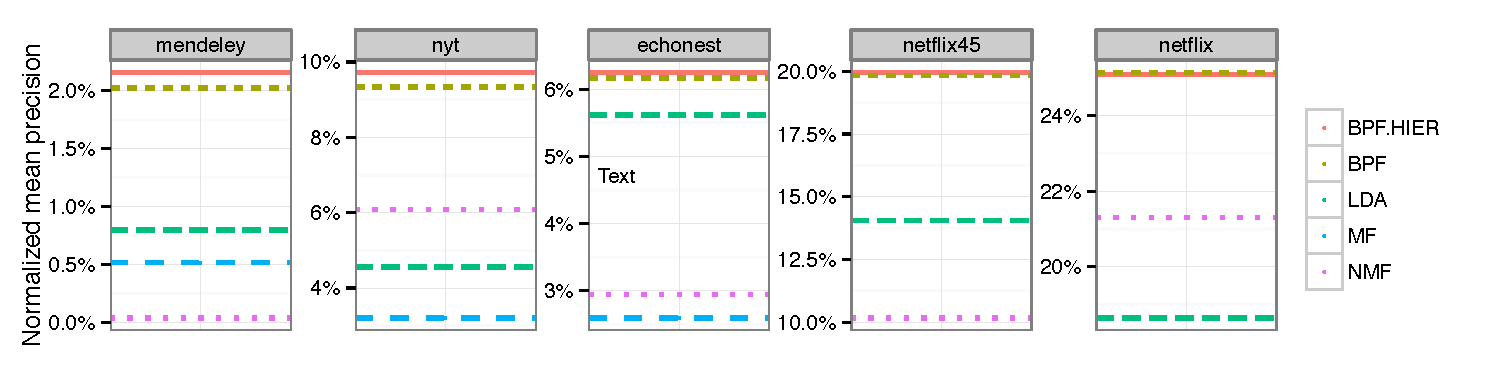
\includegraphics[width=\textwidth]{figures/mean_precision_at_10.pdf}\\
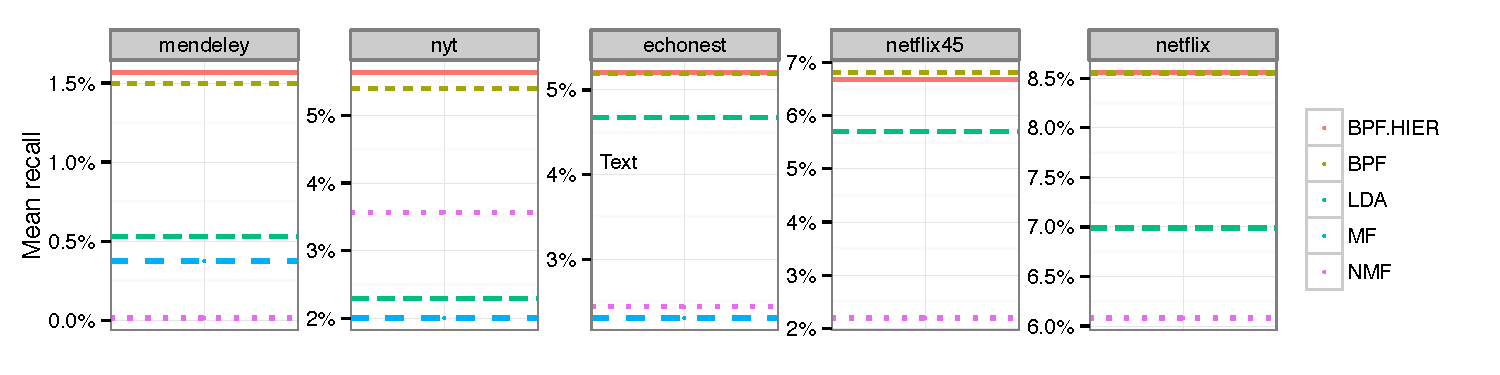
\includegraphics[width=\textwidth]{figures/mean_recall_at_10.pdf}\\
\caption{Predictive performance on datasets. The top and bottom plots
  show normalized mean precision and mean recall at 10
  recommendations, respectively.}
\label{fig:precision_recall_at_10}
\end{figure*}


%% \begin{figure*}[t!]
%% \centering
%% 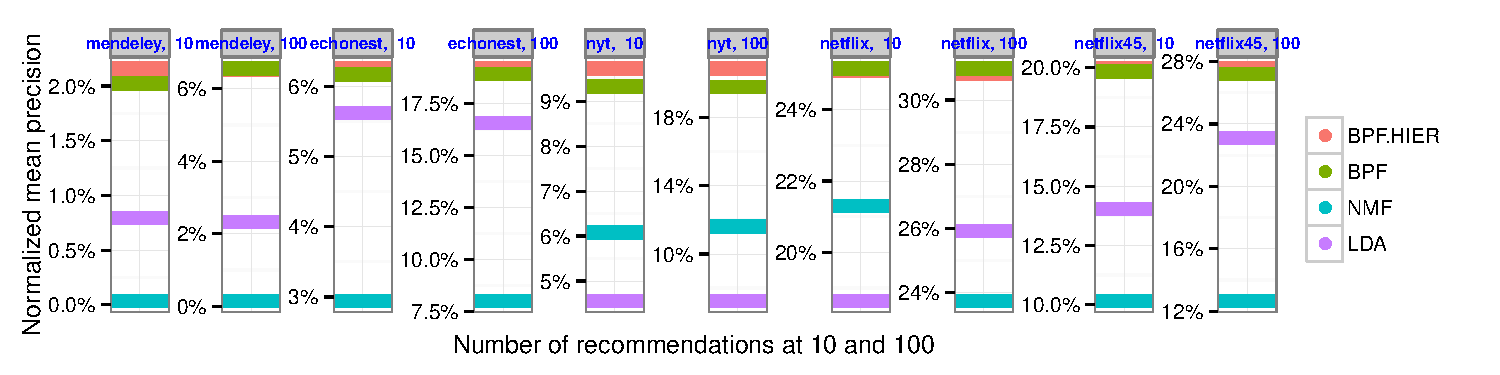
\includegraphics[width=\textwidth]{./figures/meanprecision2.pdf}\\               
%% 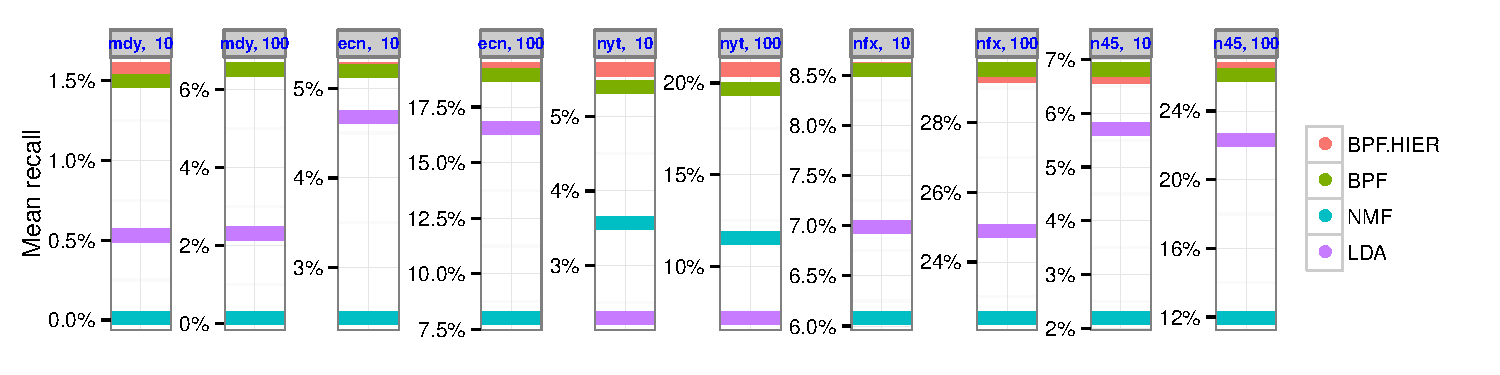
\includegraphics[width=\textwidth]{./figures/meanrecall2.pdf}\\               
%% 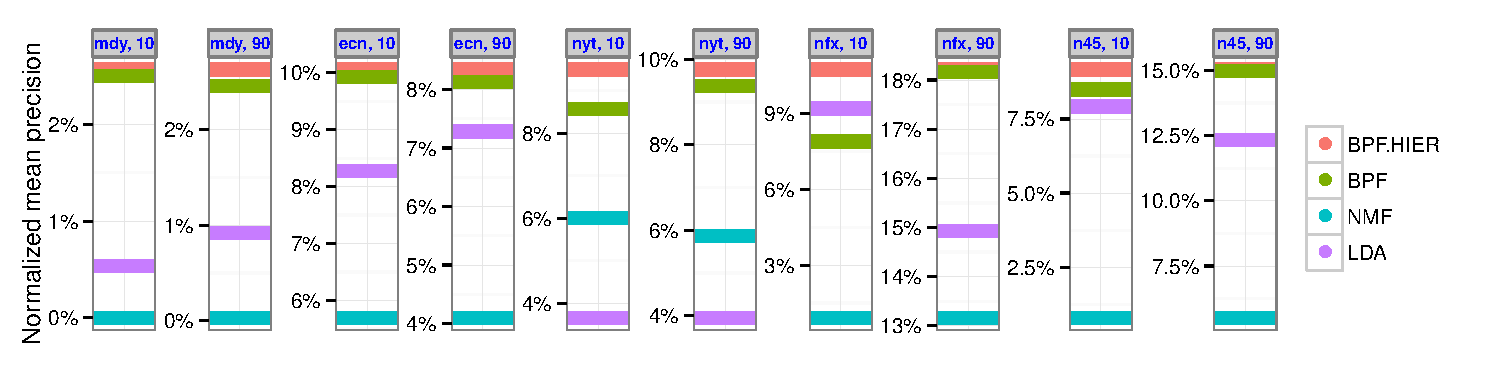
\includegraphics[width=\textwidth]{./figures/useractivity-meanprecision2.pdf}\\
%% 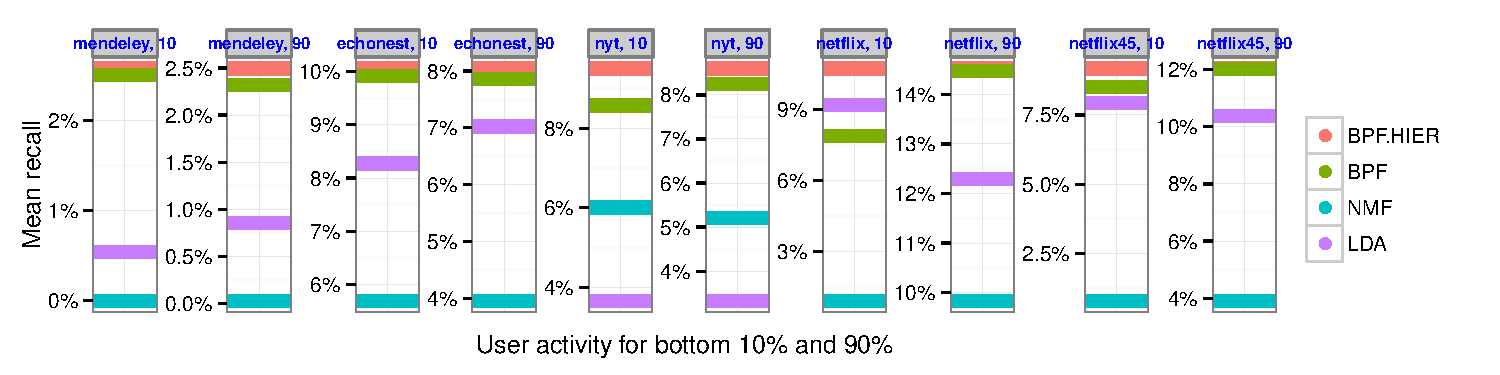
\includegraphics[width=\textwidth]{./figures/useractivity-meanrecall2.pdf}\\
%% \caption{Predictive performance on datasets. The top two plots show
%%   normalized mean precision and mean recall at 10 and 100
%%   recommendations. The bottom two plots show normalized mean precision
%%   and mean recall for the bottom 10\% and bottom 90\% of users by
%%   activity.}
%% \label{fig:precision_by_M}
%% \end{figure*}


\section{Empirical Study}
We studied the Bayesian Poisson Factorization (BPF) algorithm of
Figure~\ref{fig:batch} on a variety of large real data sets. We
demonstrate in this section that BPF definitively outperforms matrix
factorization (MF) in predictive performance on all data sets.
\begin{figure*}[th]
\centering
\subfigure[]{
  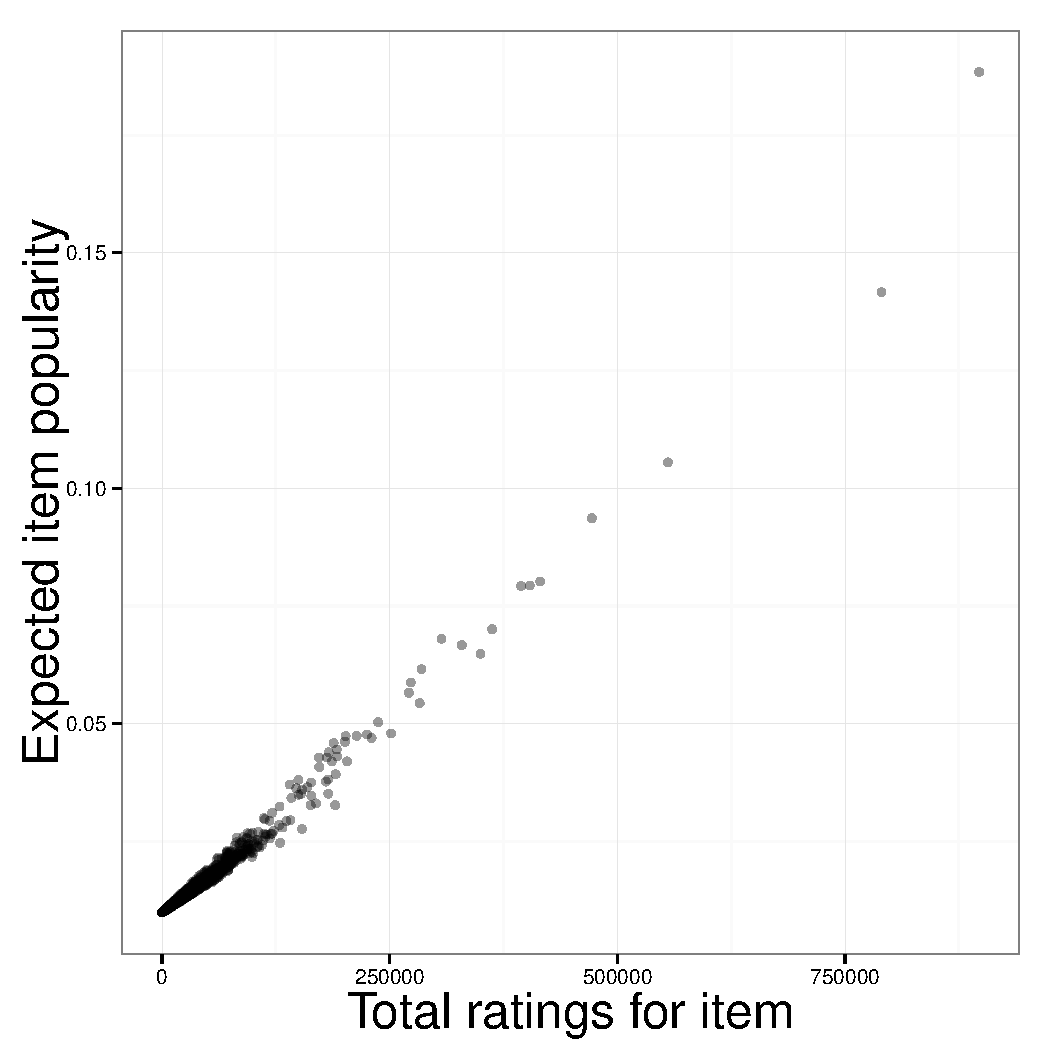
\includegraphics[width=0.45\textwidth]{./figures/nyt/itemsrate.pdf}
}
\subfigure[]{
  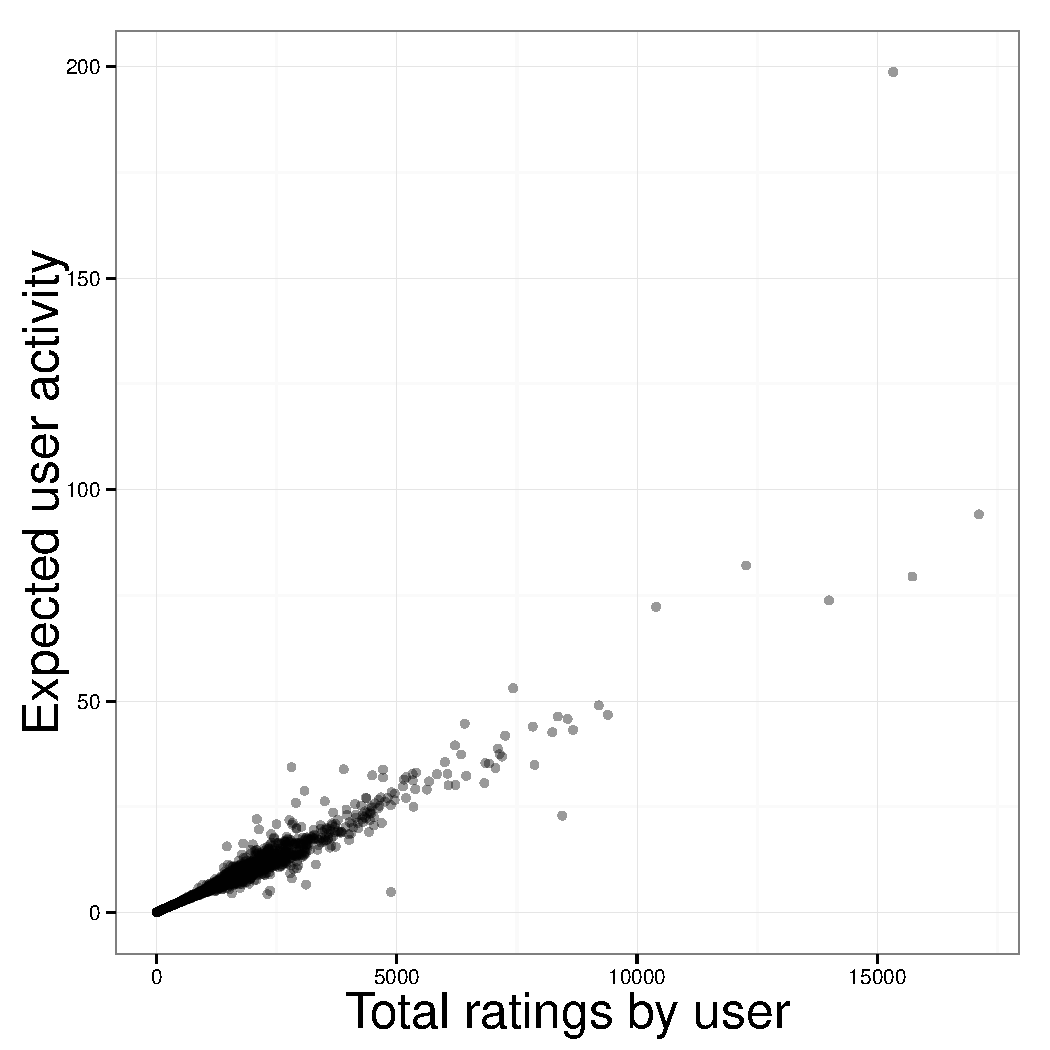
\includegraphics[width=0.45\textwidth]{./figures/nyt/userrate.pdf}
}
\caption{Popularity of articles on the NYT dataset.}
\label{fig:nyt-expl}
\end{figure*}


\begin{table*}
\centering
\caption{Most popular articles in the NYT dataset}
\begin{tabular}{|l|r|r|} \hline
Title & Expected popularity & Number of factors\\\hline
Blasts at Boston Marathon Kill 3 and Injure 100 & 0.043 & 1\\\hline
FBI Posts Images of Pair Suspected in Boston Attack & 0.042 & 1\\\hline
Bombing Inquiry Turns to Motive and Russia Trip & 0.037 & 1\\\hline
War Zone at Mile 26: 'So Many People Without Legs' & 0.025 & 1\\\hline
Suspects Seemed Set for Attacks Beyond Boston & 0.031 & 1\\\hline
In Signal Image From Boston Bombing a Father Sees His Son & 0.029 & 1\\\hline
Skeleton in British Parking Lot Hailed as Richard III & 0.027 & 4\\\hline
Surviving Suspect is Charged by US in Boston Attack & 0.027 & 1\\\hline
The Boy With A Thorn In His Joints & 0.026 & 3\\\hline
Drowned in a Stream of Prescriptions & 0.025 & 3\\\hline
\end{tabular} 
\end{table*}

{\bf Data Sets.} We study the Bayesian Poisson Factorization algorithm
in Figure~\ref{fig:batch} on several large data sets:
\begin{itemize}
\item The {\bf New York Times} data set with 1,615,675 users, 103390
  articles movies and 80,071,435 ratings.
\item The {\bf Netflix} data set~\cite{Koren:2009} with 480,000 users,
  17,770 movies and 100 million ratings is similar to MovieLens but
  significantly larger. Unlike the MovieLens data, the Netflix data
  set is highly skewed and is more realistic: Some users rate more
  than 10,000 movies, while others rate less than
  5~\cite{Salakhutdinov:2008a}.
\item The {\bf Mendeley} data set~\cite{Jack:2010} of scientific
  articles is a binary matrix of
  80,000 users and 260,000 articles, where an article is considered
  consumed by a user if it's in the user's library.
\item The {\bf Echo Nest} music data set~\cite{Bertin-Mahieux:2011} consists of 1
  million users, 385,000 distinct songs and 48 million (user, song,
  play count) triplets.
\end{itemize}

The scale and diversity of these data sets enables a robust evaluation
of our algorithm. Both the Mendeley and the Echo Nest data sets are
sparse in comparison to the movie data: only 0.001\% of the matrix of
ratings is non-zero in Mendeley, while 1\% of the ratings are non-zero
in Netflix and 4\% in MovieLens. Further, the Mendeley data set has
many more articles than users.


%% users watching movies on MovieLens~\cite{Koren:2009} and
%% Netflix~\cite{Herlocker:1999}, individuals listening to songs in the
%% Echo Nest data set~\cite{Bertin-Mahieux:2011}, and academics reading
%% scientific articles via Mendeley~\cite{Jack:2010}.


%% The MovieLens data set consists of 1 million ratings
%% from 6040 users on 4000 movies. Each movie is associated with a title
%% and a category. The Netflix data set is similar to---but significantly
%% larger than---the MovieLens data set, consisting of 100M ratings from
%% 480,000 users on 17770 movies.

{\bf Pre-processing and training.} We now describe how we the
pre-process the input data, train the model, and assess the predictive
accuracy on a held-out set.

Prior to training, we randomly select 20\% of ratings in each data set
to be used as a held-out test set comprised of items that the user
has consumed. During training, these test set observations are treated
as zeros. Additionally, we set aside 1\% of the training ratings as a
validation set and use it to determine the convergence of our
algorithm.

During training, the input to our algorithm is the count data, for
example, the movie ratings or the play count of a song. Notice that
for the Mendeley data set, the input is binary. During training, we
fix the shape and rate hyperparameters. This gives good performance on
our validation set. We find that the algorithm is insensitive to small
changes in the hyper-parameters.

%% corresponding to ratings or the play count of a song. Optionally, the
%% algorithm can transform the input count data to binary before training
%% the model.  For example, the observation $y_{ui}$ is set to one only
%% if the $u$-th user explicitly rated the $i$-th movie. (We denote the
%% algorithm that fits the transformed data, BPF-binary or BPF-BIN.)

We terminate the training process when the BPF algorithm
converges. The convergence is measured by computing the prediction
accuracy on our validation set. We approximate the probability that a
user consumed an item using the variational approximations to
posterior expectations of $\theta_u$ and $\beta_i$, and compute the
average predictive log likelihood of the validation ratings. The BPF
algorithm stops when the change in log likelihood is less than
0.0001\%.

\begin{figure*}[t!]
\centering
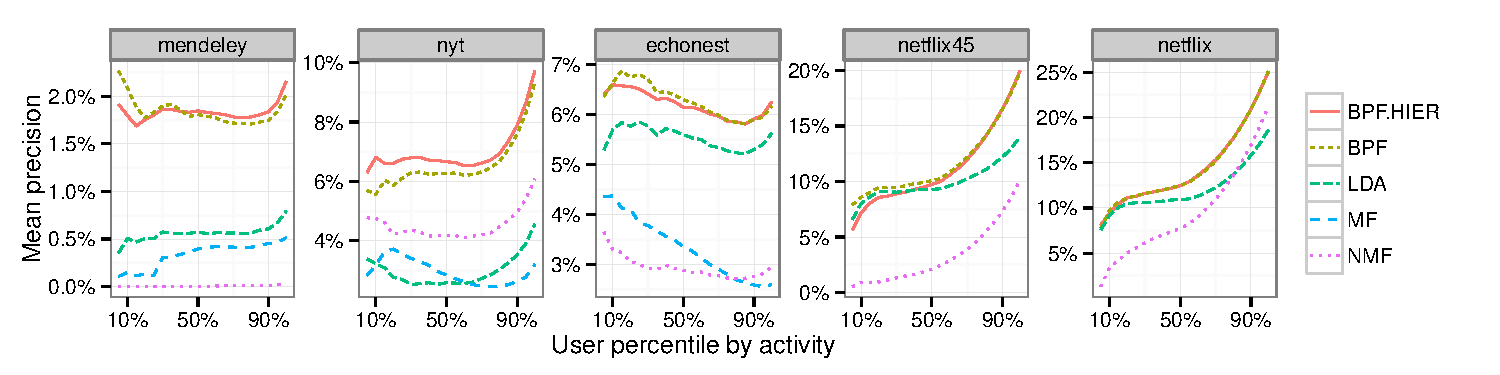
\includegraphics[width=\textwidth]{figures/mean_precision_by_user_percentile.pdf}\\
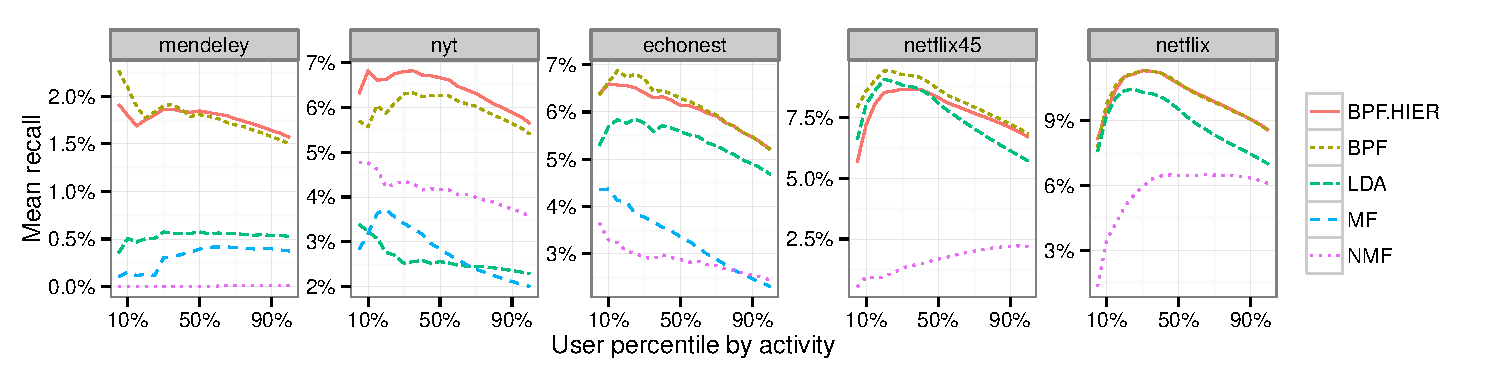
\includegraphics[width=\textwidth]{figures/mean_recall_by_user_percentile.pdf}\\
\caption{Predictive performance across users. The top and bottom plots
  show normalized mean precision and mean recall at 10
  recommendations, respectively, by user activity.}
\label{fig:precision_recall_by_user_activity}
\end{figure*}


{\bf Exploratory analysis.} The fitted model can be explored to
discover latent structure among items and users and to confirm that
the model is capturing the components in the data in a reasonable
way. For example, in \myfig{components} we illustrate the components
discovered by our algorithm on the MovieLens and the Netflix movie
ratings and the Mendeley data of users and scientific articles. For
each data set, the illustration shows the top 10 items---items sorted
in decreasing order of their expected weight $\beta_i$---from three of
the 100 components discovered by our algorithm. These components
naturally organize the movies and articles, and enable recommendation
of new items to the user.

In \myfig{movielens-illustration} we show a subset of the highly rated
movies of a user from the MovieLens data
set~\cite{Herlocker:1999}. The top 15 movies recommended to this user
using the trained BPF model, are also shown. The user's ratings are
for primarily drama movies. We movies BPF recommends closely resemble
the types of drama movies she is interested in, for example,
``Children's drama'' or ``War drama''. The expected user's $K$-vector
of weights $\theta_u$, inferred by our algorithm, is shown in
\myfig{movielens-illustration}. In our analysis, $K$ was set to
100. The $\theta_u$ are not sparse because the user's views span a
range of movies in the small data set.

{\bf Testing.} During testing, we generate the top $M$ recommendations
for each user as those items with the highest predictive score in
\myeq{score}. The ranked list of items predicted for each user
includes items in the test set, as well as items in the training set
that were zeros. We compute precision-at-$M$, which measures the
fraction of the top $M$ recommendations present in the test set,
varying $M$ from 10 to 100 items. Likewise, we compute recall-at-$M$,
which captures the fraction of items in the test set present in the
top $M$ recommendations.

%% In contrast, the Echo Nest and Mendeley data sets contain implicit
%% feedback on which songs and scientific papers users have consumed.

%% !!! prem: assume BPF-binary for now. will try to move to BPF-bias
%% where the non-binary observations are fit

{\bf Baselines.} We compare our performance against traditional matrix
factorization (MF). Ratings are modeled as
\begin{equation*}
  y_{ui} = c + a_u + b_i + \theta_u^\top \beta_i,
\end{equation*}
where $c$ denotes a global intercept term, $a_u$ captures the relative
activity of the $u$-th user, and $b_i$ accounts for the popularity of
the $i$-th item. The final term quantifies interactions between a user
and item via their K-dimensional latent factors, with $\theta_u$ specifying
the user's interests and $\beta_i$ describing the item's attributes. The
model is fit by stochastic gradient descent using the open source
Vowpal Wabbit package~\cite{Weinberger:2009} to minimize squared error
between predicted and actual ratings.

We note that while BPF takes only the non-zero observed ratings as
input, traditional matrix factorization requires that we provide
explicit zeros in the ratings matrix as negative examples. In
practice, this amounts to either treating all missing ratings as zeros
and down-weighting to balance the relative importance of observed and
missing ratings~\cite{Hu:2008p9402}, or generating negatives by
randomly sampling from missing ratings in the training
set~\cite{Dror:2012a}.  We take the latter approach for computational
convenience, employing two popular sampling schemes. In the first,
denoted MF-UNI, we sample a fixed number of negative examples
uniformly at random for each user such that there are approximately
the same number of positive and negative examples. In the second,
termed MF-POP, we sample users by activity---the number of items rated
in the training set---and items by popularity---the number of training
ratings an item received. 

For MF, we cross-validate over the gradient update step size, the
strength of an $L_2$-regularization term across all weights, and the
number of passes over the training data. This results in a reasonably
expensive grid search, from which we select
the model that performs best on the validation set for each data set.

%% \begin{figure*}[t]
%% \centering
%% \includegraphics[width=\textwidth]{./figures/precision_by_user_activity_and_method.pdf}\\
%% \label{fig:precision_by_user_activity}
%% \caption{Precision at 100 recommendations by user activity across data sets and methods.}
%% \end{figure*}

%% \begin{figure*}
%% \centering
%% 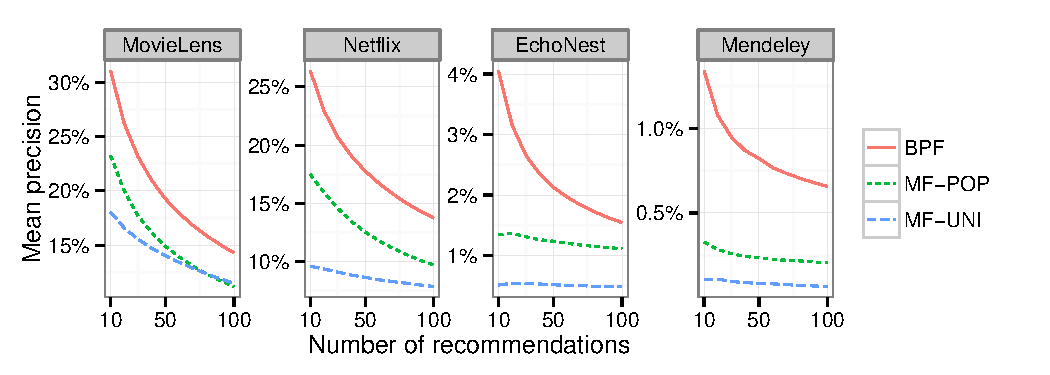
\includegraphics[width=\textwidth]{../output/figures/echonest_and_mendeley/mean_precision_by_method.pdf}\\
%% \includegraphics[width=\textwidth]{../output/figures/echonest_and_mendeley/precision_by_user_activity_and_method.pdf}\\
%% \includegraphics[width=\textwidth]{../output/figures/echonest_and_mendeley/mean_coverage_by_method.pdf}\\
%% \end{figure*}

%% {\bf Results and analysis.} \myfig{precision_by_M} shows the mean
%% precision of the BPF and the MF algorithm as we vary $M$, the number
%% of recommendations. As shown in \myfig{precision_by_M}, BPF
%% outperforms MF on all data sets by a sizeable margin---as much as 8
%% percentage points. Likewise, BPF shows similar gains in recall over
%% traditional MF approaches, indicated in \myfig{recall_by_M}. A
%% relatively high fraction of items recommended by BPF are found to be
%% relevant, and many relevant items are recommended.

%% We also study precision as a function of user activity to investigate
%% for which kinds of users the algorithm performs
%% well. \myfig{precision_by_user_activity} highlights the results in
%% further detail, showing the precision at 100 recommendations for users
%% of varying activity. BPF provides increasingly better performance for
%% more active users.  On the Mendeley data set, BPF performs better for
%% users with less than 1000 articles (BPF does better over all.)  On all
%% other data sets, BPF performs better than MF with all types of users.

%% In all results, MF-POP outperforms MF-UNI, which is indicative of
%% problems with the squared loss objective approximated by MF-UNI.

%% As expected, we see that BPF provides
%% increasingly better recommendations for more active users, and that
%% BPF outperforms MF on the Netflix, MovieLens, and Echo Nest data sets
%% by this measure as well as mean precision across all users.

%% On the Mendeley data set, BPF performs better for users with less than
%% 1000 articles in their library, but MF has better precision than BPF for
%% the small set of users with more than 1000 papers in their library. 

%% !!! prem: need to confirm by looking at actual values; investigate
%\newpage

\begin{figure*}
\centering
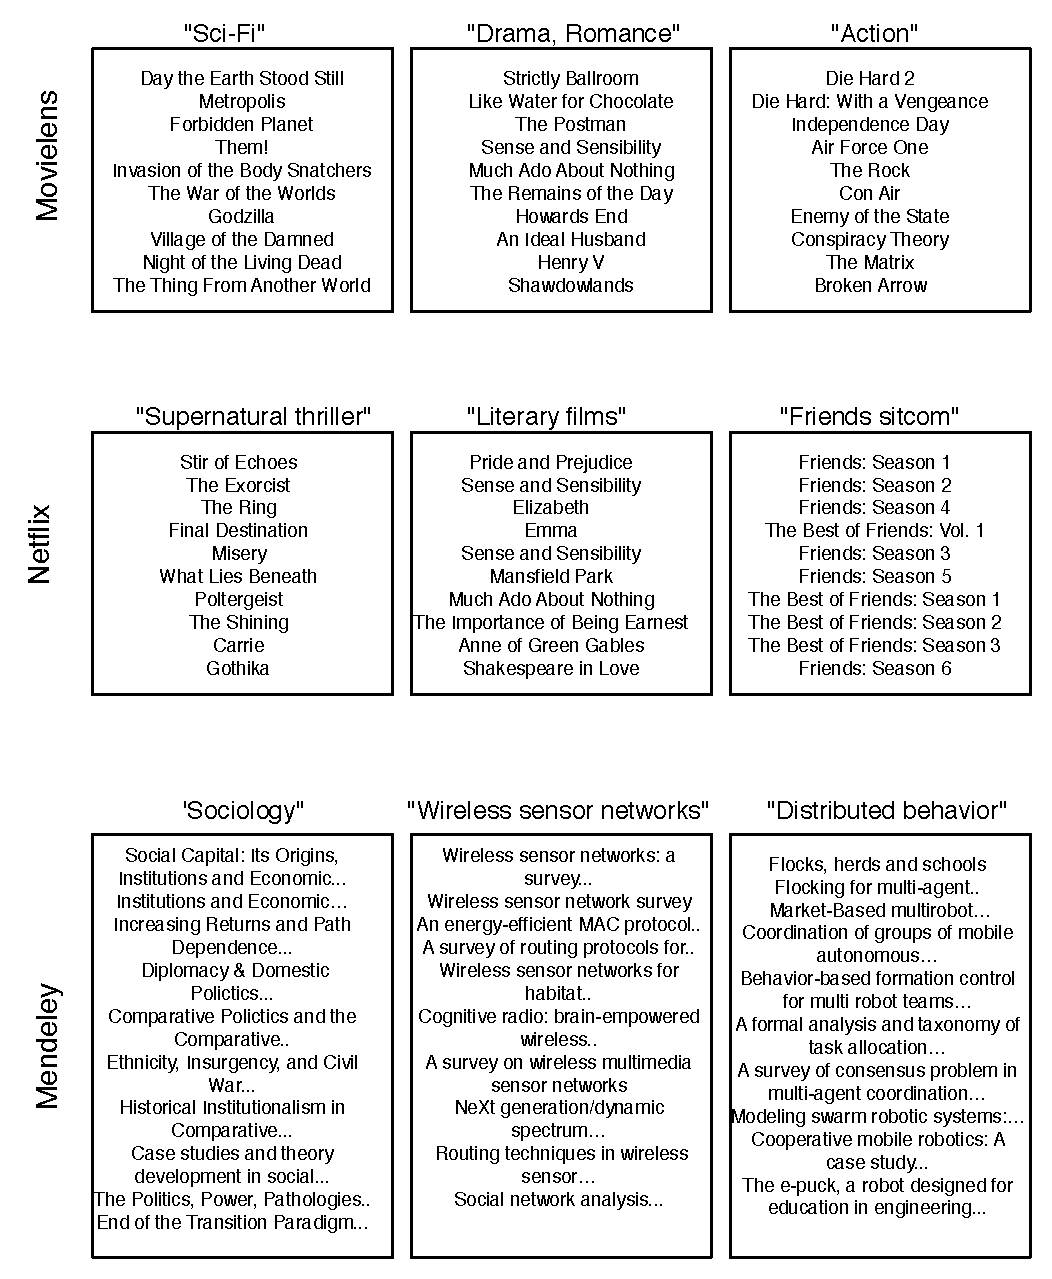
\includegraphics[width=\textwidth]{./figures/components.pdf}
\caption{The top 10 items by the expected weight $\beta_i$ from three
  of the 100 components discovered by our algorithm.}
\label{fig:components}
\end{figure*}


\section{Discussion}
We have demonstrated that Poisson factorization is an efficient and
effective means of generating high quality recommendations across a
variety of data sets ranging from movie views to scientific article
libraries. It significantly outperforms a number of leading methods in
modeling implicit behavior data without the need for ad hoc
modifications. Variational inference for HPF scales to massive data
and differs from traditional methods in its ability to capture the
heterogeneity amongst users and items, accounting for the wide range
of activity and popularity amongst them, respectively. The HPF
algorithm is a robust, off-the-shelf tool, providing high accuracy
even with fixed hyperparameter settings.

%%% recsys-prem !!! added note about SVI here (removed from intro)

Finally, we emphasize that HPF is more than just one method---it is
the simplest in a class of probabilistic models with these properties,
and has already been extended to a combined model of article content
and reader ratings~\cite{gopalan2014content}, and a Bayesian
nonparametric model that adapts the dimensionality of the latent
representations~\cite{gopalan2014bayesian}.

A notable innovation in Gaussian MF is the algorithm
of~\cite{Hu:2008p9402} that explicitly downweights zeros using
confidence parameters. We presented the empirical study in this paper
comparing to the Gaussian MF with subsampled
zeros~\cite{Koren:2009}. Our ongoing work includes bringing the
confidence-weighting of~\cite{Hu:2008p9402} into HPF.
%% To provide a fair
%% comparison to the algorithm of ~\cite{Hu:2008p9402} we need to bring
%% the confidence-weighting of~\cite{Hu:2008p9402} into HPF. 
This will allow downweighting of the zeros beyond that provided
implicitly by Poisson factorization. Our initial experiments show that
even without the downweighting, HPF provides better predictive
performance (measured using the mean rank of recommended items) for
all but the ``heaviest'' portion of the long tail of items, consisting
of the least popular items in the data sets.

%% we present our empirical study
%% without hu et al., but discuss the need to downweight the zeros on
%% even heavier tailed data sets.  we can note that PF dominates gaussian
%% factorization everywhere, but one innovation in gaussian factorization
%% is hu et al. (even if it is unprincipled).  we can talk about ``pilot
%% studies'' against hu et al. which found better performance in most
%% cases, and always for the more popular items.  an area of future work
%% to bring its intuition into PF.

%% This will allow us to provide a fair comparison to the Gaussian
%% MF with downweighted zeros~\cite{Hu:2008p9402}. 

%% , we are comparing to the Gaussian
%% MF with downweighted zeros~\cite{Hu:2008p9402}.

%%  included the 

%% Future work 

%% exploring modifications to BPF to incorporate
%% additional features---e.g., user and item metadata---as well as
%% stochastic inference to scale to massive data sets and Bayesian
%% non-parametric extensions~\cite{Zhou:2012}.


%% In settings where there are many more items than the typical user
%% can consume, unobserved consumption is likely explained by finite
%% attention, as opposed to an active dislike for the associated
%% content. Likewise, a user's choice in selecting a particular set of
%% items amongst the many available options is a relatively strong
%% indicator of her interests. BPF captures these features of sparse user
%% data via the Poisson likelihood, which appropriately balances strong
%% signals of consumption with weaker signals of unobserved activity.

%% Conveniently, the same Poisson likelihood also leads to
%% computationally efficient inference on sparse data sets, as it requires
%% evaluation of only the consumed user-item pairs, which comprise a
%% small fraction of all possible observations. This avoids the issue
%% faced by traditional matrix factorization in down-weighting or sampling
%% negative examples during training. In addition to this computational
%% advantage, BPF empirically outperforms classical MF across a wide array
%% of data sets---from movies to music to scientific articles---in
%% recommending relevant content to users.

%Future work includes exploring modifications to BPF to incorporate
%additional features---e.g., user and item metadata---as well as
%stochastic inference to scale to massive data sets.



%% There has also been significant research on Bayesian nonparametric
%% Poisson factor models. Using a Beta-Negative-Binomial process prior
%% for Poisson factor analysis the authors of ~\cite{Zhou:2012}
%% demonstrate that NMF, LDA and GaP are special cases of a finite
%% approximation to their model. Inference for the models
%% in~\cite{Zhou:2012} do not scale to the size of datasets we consider
%% here.


\bibliographystyle{abbrv}
\bibliography{bib}

\appendix

\section{Poisson factorization and LDA}

We show that LDA is equivalent to Poisson factorization, conditioned
on the per-user sums and where the item weights are constrained to sum
to one (across items, for each component).  To show this fact we
appeal to the relationships between the Gamma and Dirichlet
distributions and between the Poisson and multinomial distributions.

LDA is a mixed-membership model of word counts.  There are a set of
``topics'' $\gamma_{1:K}$, distributions over a fixed vocabulary, and
each document exhibits those topics with different proportions.
Applied to the setting here, the vocabulary is the set of items; each
user is a ``document'', represented as a sparse vector of item counts;
a topic is a distribution over items, $\sum_{j} \gamma_{kj} = 1$; each
user's topic proportions are denoted $\pi_u$, where $\sum_k \pi_{uk} =
1$.  User/item data, treated as documents, was one of the original
applications of LDA~\cite{Blei:2003b}.

To see the connection to Poisson factorization, we take the
``multinomial PCA'' perspective of LDA~\cite{Buntine:2004}.  Let
$\Gamma$ be the $K \times I$ matrix of topics, where each row
$\gamma_k$ is a distribution over $I$ items.  Recall that the
Dirichlet distribution is a distribution over the simplex,
non-negative vectors that sum to one.  For a distribution on the
$K$-simplex, the Dirichlet parameter is a positive $K$-vector.  The
generative process for LDA is
\begin{eqnarray*}
  \gamma_k \sim & \dir(\eta) & \quad k \in \{1, \ldots,
  K\} \\
  \pi_u  \sim &\dir(\alpha) & \quad u \in \{1, \ldots, U\}
  \\
  y_u \sim & \mult(n_u, \pi_u^\top \Gamma). & \quad u \in
  \{1, \ldots, U\}.
\end{eqnarray*}
This process conditions on $n_u$, the sum of the counts for user $u$.
Further, we assume exchangeable Dirichlets, that is, the
hyperparameters $\alpha$ and $\eta$ are scalars repeated $K$ and $I$
times, respectively, for their corresponding Dirichlet parameters.
This generative process is different from but equivalent to the
original process for LDA~\cite{Blei:2003b}.

Before connecting LDA and Poisson factorization, we articulate the
relationship between the Gamma and Dirichlet and between the Poisson
and multinomial.  The relationship between the Dirichlet and Gamma
distributions is that we can write a Dirichlet random vector as a
normalized vector of independent Gammas.  Let $\pi$ be a
$K$-dimensional simplex vector and let $\alpha$ is a positive
$K$-vector.  If we generate $\pi$ from the following two-stage
process,
\begin{eqnarray*}
  \theta_k &\sim& \gam(\alpha_k, 1) \\
  \pi_k &=& \frac{\theta_k}{\sum_{j} \theta_j},
\end{eqnarray*}
then $\pi \sim \dir(\alpha)$.

The relationship between the Poisson and multinomial is that a set of
Poisson variables, conditioned on their sum, is a
multinomial~\cite{Johnson:2005}.  Let $z_{1:K}$ be a set of Poisson
variables, each with different rates $\mu_{1:K}$.  Conditioned on
their sum $n = \sum_k z_k$, the joint distribution of $z_{1:K}$ is a
multinomial (giving a vector of counts) whose proportions are the
normalized rates,
\begin{equation*}
  z \sim \mult\left(n, \pi \right)
\end{equation*}
where $\pi_k = \mu_k / \sum_j \mu_j$.

With these two facts in hand, we can show that LDA is a type of
Poisson factorization.  First, we re-parameterize the Dirichlet topic
proportions with Gamma distributions,
\begin{eqnarray*}
  \theta_{uk} &\sim& \gam(\alpha, 1) \\
  \pi_{uk} &=& \theta_{uk} / \textstyle \sum_{j} \theta_{uj}.
\end{eqnarray*}
Second, we note that $y_u$ coming from a multinomial is equivalent to
a conditional bank of Poissons (denoted by $\poisson_{n_u}$),
\begin{equation*}
  y_u \g n_u \sim \poisson_{n_u}(\pi_u^\top \Gamma).
\end{equation*}
This conditional Poisson is equivalent to any other with the rates
scaled by a constant.  We can thus use the original Gamma variables
$\theta_{uk}$ because $\pi$ is simply scaled by its sum,
\begin{equation*}
  y_u \g n_u \sim \poisson_{n_u}(\theta_u^\top \Gamma).
\end{equation*}
Note that we cannot symmetrically scale by a Gamma representation of
$\beta_{ik}$ because the vector $\gamma_{\cdot i}$, which are the
per-topic probabilities for a fixed item, cannot be represented by a
normalized Gamma.  (Rather, it is the topics themselves, across words,
which are normalized Gammas.)

In summary, LDA is a form of Poisson factorization where (a) the
scaling parameter on the gamma priors is fixed to be one (b) we
condition on the marginal sums for each user (c) the per-item weights
are scaled to sum to one for each component.

% dmb: consider adding a cite to tina's paper.  note: this justifies
% using LDA where it might seem "unnatural" to think about bags of
% words

\end{document}
